% Copyright (c) 2014,2016 Casper Ti. Vector
% Public domain.

\chapter{Storage Layer}
HybriG将图数据分开存储在Titan和HBase中。具体地,如果两点之间有相同label的重边,HybriG会在Titan中这两点间建立一条该label的边,将对应重边的数据都存储在HBase中的一个表,不妨称其为边表。每条边一行,行键是Titan图中分配的边id拼接上重边的主键,单元格的值则存放具体边的内容。重边的主键是这样定义的:在两点间同label的重边中,如果有一个属性能唯一确定一条边,则选该属性作为主键。比如交易关系的时间戳,两个人在同一个时间点只能发生一次交易,因此该时间戳可以唯一确定两人间的一次交易。如果某种label的边没有属性能唯一确定一条重边,则选该数据插入的时间戳作为主键。
在HBase边表中,同label的重边数据的行键都有相同的前缀(即Titan中的边id),由于HBase中的数据是按行键排序的,它们在HBase中有相邻的位置。同label的重边经常会被同时检索,这种设计使得一次顺序扫描便可得到所有同label的重边。另外,HybriG利用Titan中边上的属性记录一些统计信息,如原图中实际有几条这样的重边,或者边上某个属性值的求和等,这些统计信息可以根据业务定制,用来加快业务相关的查询,不用再遍历相关的边。

\begin{figure}[htbp]
\centering
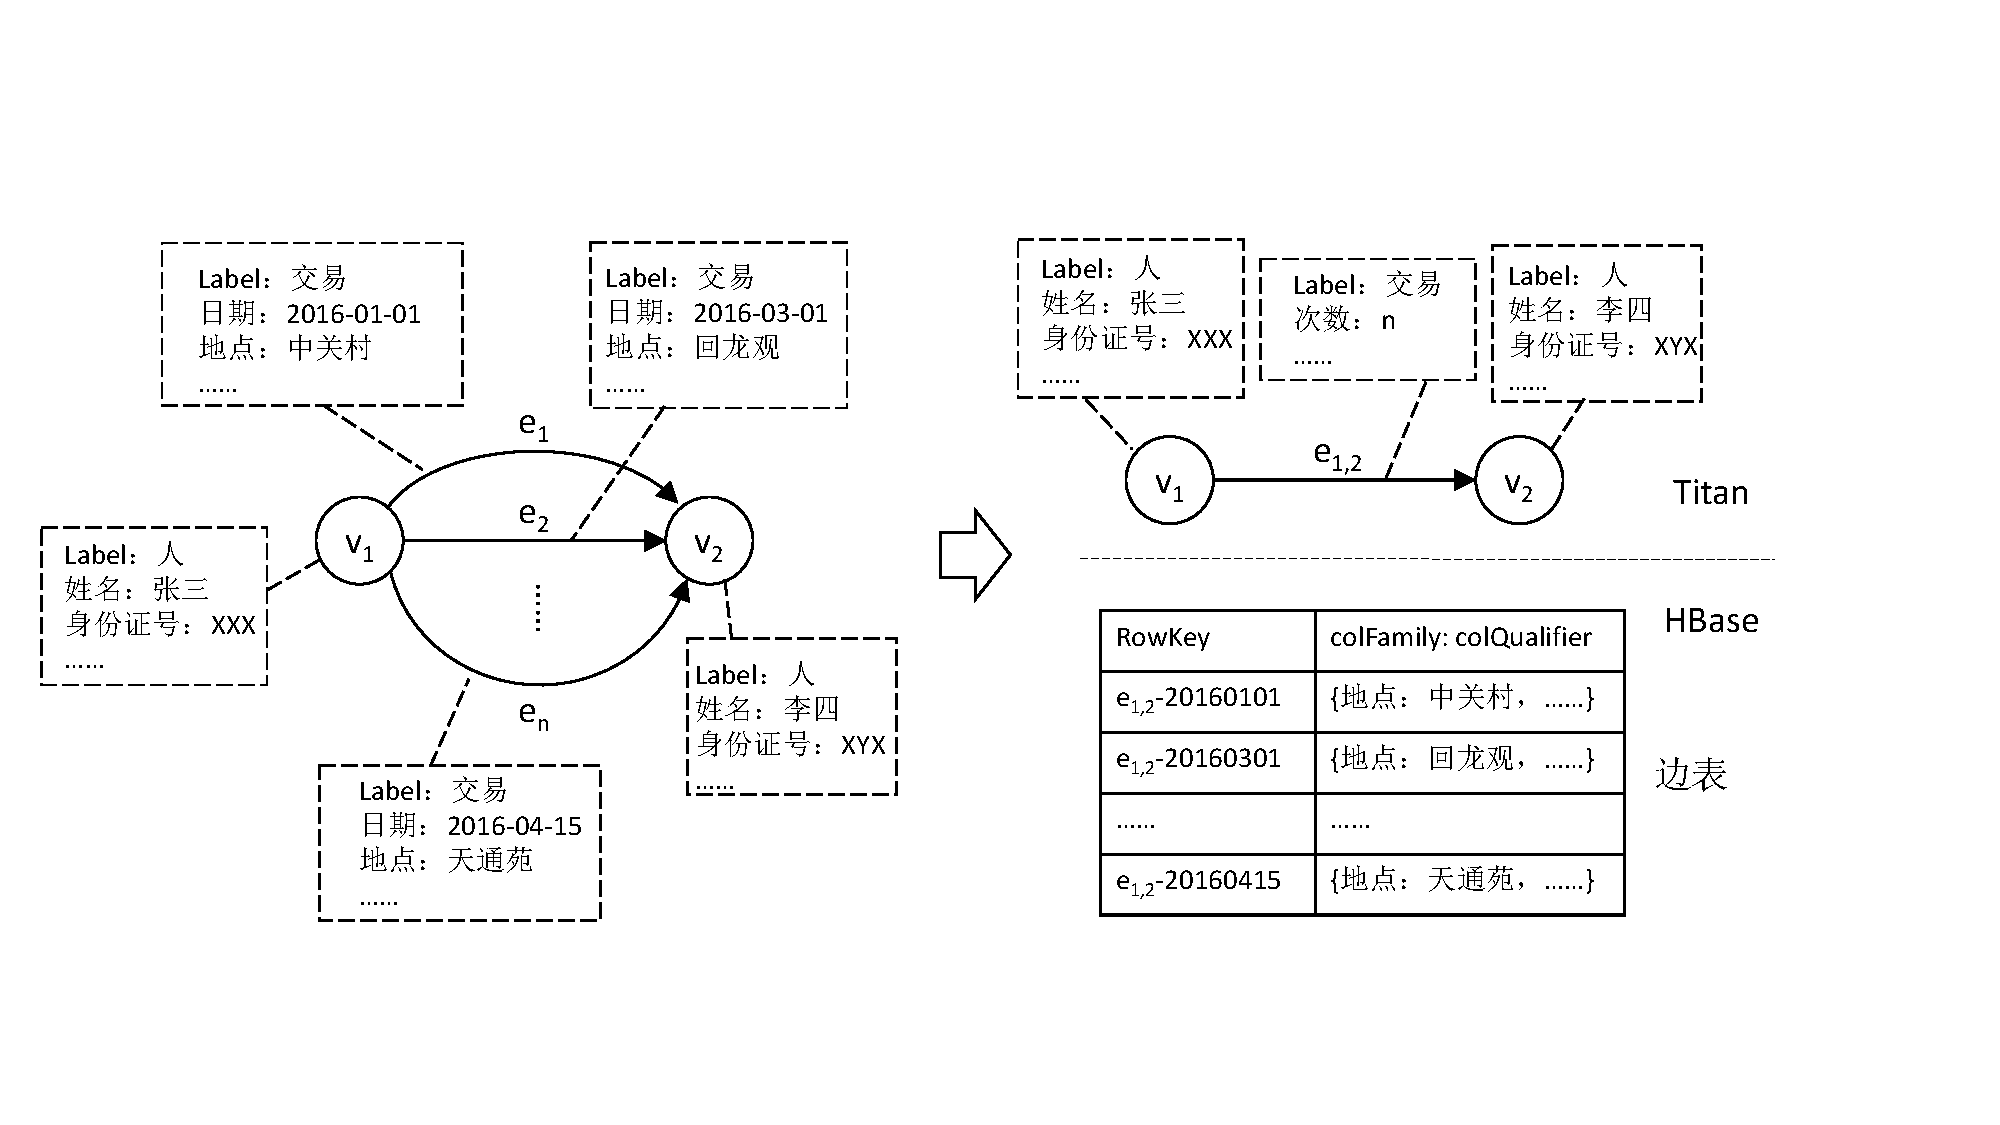
\includegraphics[width=150mm]{fig/storage_layer.pdf}
\caption{HybriG存储示例。左图为原始数据的属性图,右图为数据在Titan和HBase边表的存储情况。}
\label{fig:storage_layer}
\end{figure}

图 \ref{fig:storage_layer}是数据存储的一个示例,左边是实际要存储的图数据, e1、e2、…、en都是label为“交易”的重边,表示两人的所有交易记录。右边是数据在Titan和HBase中的存储情况。Titan中只存一条label为“交易”的边,该边有一个属性记录实际的边数。利用这条边的id作为前缀,拼接上重边的主键(交易的时间戳)作为HBase的行键,将每条边的数据都存入对应的单元格中。
本文在引言中提到了一种避免产生重边的建模方式,即将所有同label的重边合并为一条边来表示,边上存储这些重边的所有数据。HybriG架构与其有相似之处,但本质区别是边集元素的数据粒度仍是每条重边,不会将多条重边的数据作为一个单元来处理。在HybriG中每条边的数据独占HBase边表中的一行,因此每条边的相关操作都会更加高效。得益于HBase的高可扩展性,这种存储方式的性能也不会受制于数据规模的增长。而前述建模方式将所有重边的数据合并在一条边中存储,当重边量级巨大时,对每条边的操作势必更加低效。

\begin{figure}[htbp]
\centering
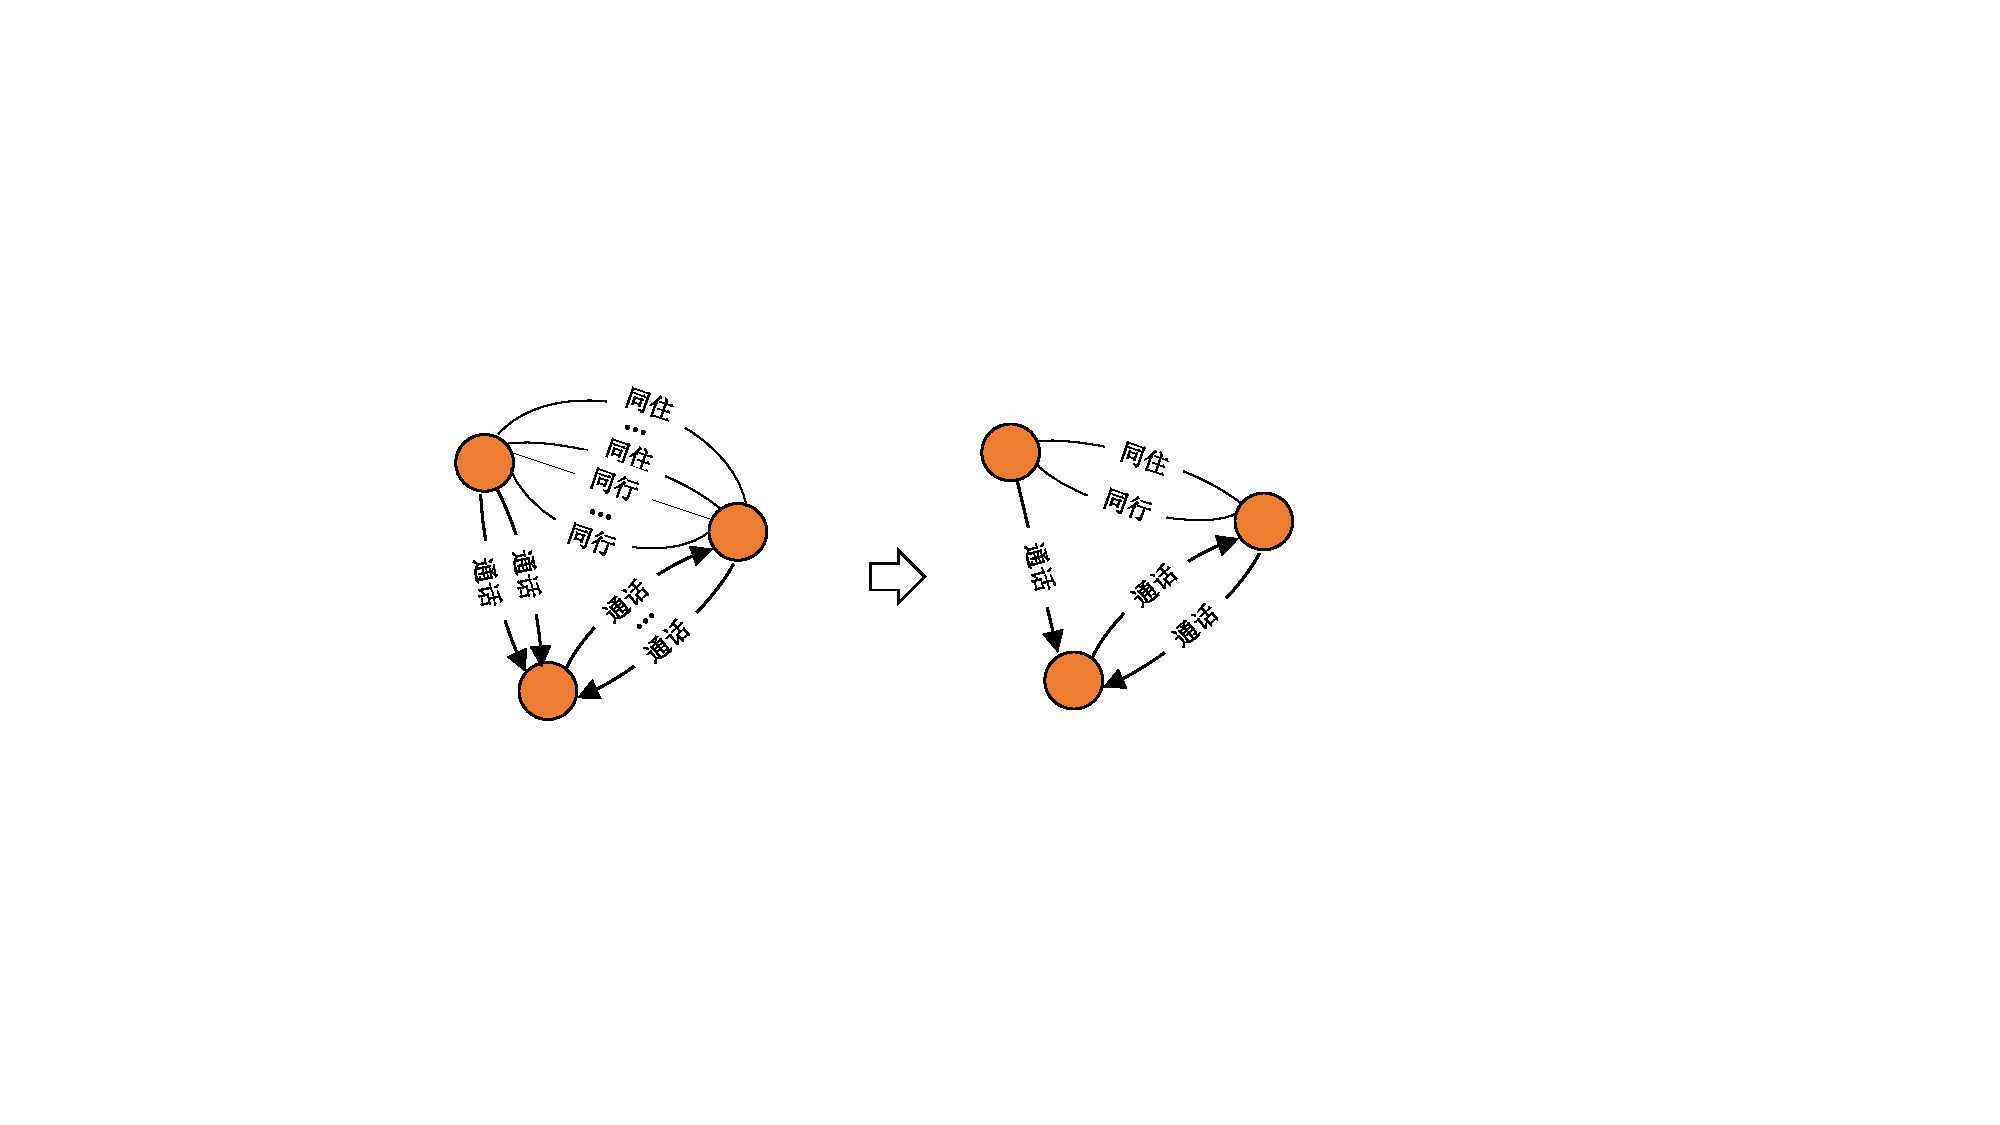
\includegraphics[width=100mm]{fig/merge_edges.pdf}
\caption{合并同label重边示意。左图为实际数据图,右图为Titan中的存储示意图。无向边中的重边是指端点对应相同的两条或多条边,有向边中的重边是指起点和终点对应相同的两条或多条边。}
\label{fig:merge_edges}
\end{figure}

HybriG采用的是合并同label的重边,而不是所有的重边,这仍是基于数据粒度的考虑。图\ref{fig:merge_edges}是合并相同label重边后Titan的图示例(在HBase边表中的重边数据未显示)。在实际应用场景中,经常需要根据具体的关系种类(label)来进行邻域点集查找,对于具体边数据的查询也常按label进行。因此合并相同label的重边设计可以使很多查询在Titan中就得到满足,不需要再涉及HBase边表。


% vim:ts=4:sw=4
